\section{Euler: The Bridge from Circles to Exponentials (1748)}

If Barrow saw curves as geometric entities—measured by tangents and areas—then \textbf{Leonhard Euler} saw them as expressions waiting to be simplified. Where Barrow drew triangles, Euler wrote formulas. Where Barrow relied on proportions, Euler invoked a new kind of mathematical poetry:  
\[
e^{ix} = \cos(x) + i \sin(x)
\]

With this single equation, Euler didn’t just connect exponentials and trigonometric functions—he redefined how we think about motion, oscillation, and periodicity.

\subsection{From Circles to Signals}

For centuries, \textbf{trigonometry} was inseparable from geometry. Sines and cosines were lengths of lines inside a circle—tools for navigators, architects, and astronomers. But Euler asked a different question:

\begin{quote}
\textit{What if circular motion could be described not by shapes, but by growth and rotation in the complex plane?}
\end{quote}

By extending the exponential function into the realm of imaginary numbers, Euler discovered that rotation itself could be encoded algebraically. The endless sweep of a circle became a natural consequence of exponential behavior—an elegant spiral through the fabric of numbers.

\subsection{Analysis Over Diagrams}

Where Barrow’s world was drawn with careful hands, Euler’s was written with flowing symbols. He replaced geometric constructions with analytic expressions:

\[
\cos(x) = \frac{e^{ix} + e^{-ix}}{2}
\quad \text{and} \quad
\sin(x) = \frac{e^{ix} - e^{-ix}}{2i}
\]

These identities didn’t just simplify calculations—they unlocked entirely new ways of thinking:

\begin{itemize}
    \item Oscillations could now be treated as combinations of exponential functions.
    \item Problems in mechanics, astronomy, and later electrical engineering were transformed by this shift from angles to exponents.
    \item The door to \textbf{Fourier analysis}, signal processing, and quantum mechanics stood open—whether Euler knew it or not.
\end{itemize}

\begin{figure}[H]
    \centering
    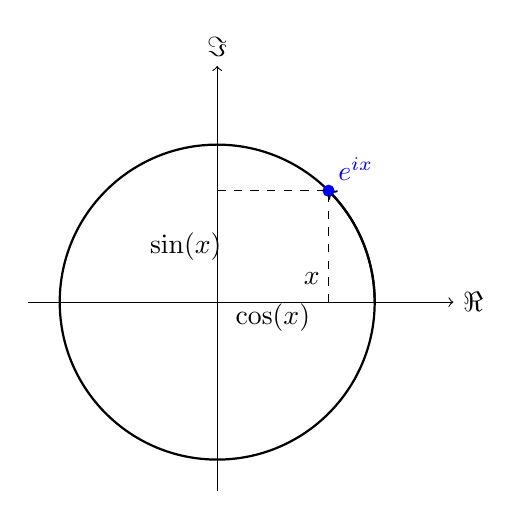
\begin{tikzpicture}[scale=2]
      % Draw unit circle
      \draw[thick] (0,0) circle (1);
      \draw[->] (-1.2,0) -- (1.5,0) node[right] {$\Re$};
      \draw[->] (0,-1.2) -- (0,1.5) node[above] {$\Im$};
      
      % Angle arc
      \draw[thick, ->] (1,0) arc (0:45:1);
      \node at (0.6,0.15) {$x$};
      
      % Point on circle
      \filldraw[blue] ({cos(45)},{sin(45)}) circle (1pt) node[above right] {$e^{ix}$};
      
      % Cosine projection
      \draw[dashed] ({cos(45)},0) -- ({cos(45)},{sin(45)});
      \node at ({cos(45)/2}, -0.1) {$\cos(x)$};
      
      % Sine projection
      \draw[dashed] (0,{sin(45)}) -- ({cos(45)},{sin(45)});
      \node at (-0.2,{sin(45)/2}) {$\sin(x)$};
    \end{tikzpicture}
    \caption{Euler’s Formula: Rotating around the unit circle becomes an exponential journey in the complex plane.}
\end{figure}

\subsection{The End of Geometric Dependence}

Euler’s work marked a turning point:

\begin{center}
\textit{Where Barrow needed diagrams, Euler needed only \( e^{ix} \).}
\end{center}

Trigonometry was no longer bound to the compass and straightedge. It had been absorbed into the algebra of exponentials—compressed into a form that could travel far beyond the page, into differential equations, wave mechanics, and the heart of modern analysis.

\vspace{1em}

Euler didn’t just compute faster—he changed what it meant to \textbf{understand} periodic motion.  
A circle, once a purely geometric object, became a manifestation of exponential behavior—an idea that still powers mathematics today.
